% AgentGS English manuscript translated from AgentGS-revisebycjx(5)_融合优化稿_20261009.docx.
\documentclass[sigconf,anonymous]{aamas}
% For the camera-ready version: \documentclass[sigconf]{aamas}

\usepackage{balance}
\usepackage{tabularx}
\usepackage{algorithm}
\usepackage{algpseudocode}
\usepackage{placeins}
\makeatletter
\setkeys{aamas.cls}{balance=false}
\makeatother
\graphicspath{{figures/}}

% Visible draft placeholders; replace each item when the missing material is ready.
\newcommand{\drafttodo}[1]{\textbf{[TODO: #1]}}
\newcommand{\papersection}[2]{Section~\ref{#1}}

% Official AAMAS 2027 copyright metadata.
\makeatletter
\gdef\@copyrightpermission{
  \begin{minipage}{0.2\columnwidth}
   \href{https://creativecommons.org/licenses/by/4.0/}{
\includegraphics[width=0.90\textwidth]{by}}
  \end{minipage}\hfill
  \begin{minipage}{0.8\columnwidth}
   \href{https://creativecommons.org/licenses/by/4.0/}{This work is licensed under a Creative Commons Attribution International 4.0 License.}
  \end{minipage}
  \vspace{5pt}
}
\makeatother

\setcopyright{ifaamas}
\acmConference[AAMAS 2027]{Proc.\@ of the 26th International Conference
on Autonomous Agents and Multiagent Systems (AAMAS 2027)}{3--7 May 2027}{Hanoi, Vietnam}{M.~Baldoni, F.~Fang, W.~Yeoh, N.~Yorke-Smith (eds.)}
\copyrightyear{2027}
\acmYear{2027}
\acmDOI{}
%\acmPrice{}
\acmISBN{}

% TODO: replace with the OpenReview submission identifier.
\acmSubmissionID{TBD}
\submissionType{Research Paper Track}

% DOCX paragraphs 000--001. Author names and affiliations were not supplied.
\title[AgentGS]{AgentGS: Empowering Earth Science Agents with Plan Composition and Completion over Skill Hypergraphs}
\author{Anonymous Author(s)}
% TODO: supply authors, affiliations, and emails for the camera-ready version.

\begin{CCSXML}
<ccs2012>
<concept><concept_id>10010147.10010178.10010179</concept_id><concept_desc>Computing methodologies~Intelligent agents</concept_desc><concept_significance>500</concept_significance></concept>
<concept><concept_id>10010147.10010178.10010199</concept_id><concept_desc>Computing methodologies~Planning and scheduling</concept_desc><concept_significance>300</concept_significance></concept>
</ccs2012>
\end{CCSXML}
\ccsdesc[500]{Computing methodologies~Intelligent agents}
\ccsdesc[300]{Computing methodologies~Planning and scheduling}

% DOCX paragraph 003.
\begin{abstract}
Complex geoscientific tasks often require multiple tools to work together and exchange intermediate results across computational steps. Existing methods commonly plan around specific tools, tying workflows to particular implementations, whereas reusing entire strategies makes it difficult to combine local steps from different strategies according to task requirements. We present AgentGS, a method for capability composition and tool orchestration over skill hypergraphs. AgentGS uses a three-layer Skill--Capability--Tool representation to decouple task strategies, reusable operations, and concrete tools, allowing it to organize an operational workflow before selecting its implementations. The skill hypergraph connects strategies through shared capabilities and provides a structured basis for composition across strategies. Given selected strategies, the system expands their required operations and prerequisite steps. When the current operation chain lacks necessary intermediate steps, it searches for feasible connecting branches along dependencies declared by other strategies. By jointly checking step dependencies, data compatibility, and tool availability, the system incorporates branches that satisfy the constraints without ambiguity, thereby reusing local steps from other strategies. It then selects concrete tools, propagates task data and intermediate results, and locally recovers failed steps. AgentGS can also organize newly composed capability workflows into candidate Skills for subsequent registration and reuse. On GeoToolEval, which contains 603 evaluation records across ten geoscientific domains, AgentGS achieves a mean Final Answer Score (FAS) of 0.8731. Ablation experiments show that hierarchical planning and missing-capability completion both improve task performance, with prerequisite expansion, capability completion, and execution recovery being particularly helpful for multistep tasks.
\end{abstract}

% DOCX paragraph 004.
\keywords{LLM Agents, Compositional Planning, Tool Orchestration, Skill Hypergraph, Scientific Agent}

\begin{document}
\maketitle

\section{Introduction}
\label{sec:introduction}

From climate change and critical minerals to energy resources and disaster risk, Earth science seeks to derive testable scientific conclusions from observational data. These research frontiers are data intensive, computationally demanding, and interdisciplinary. Geoscientific research is shifting from traditional empirical inference and mechanistic simulation toward predictive systems science driven jointly by big data and artificial intelligence~\cite{zheng2025frontiers}. In this emerging paradigm, research capability depends not only on the scale of data and models, but also on the ability to organize distributed data, tools, and methods into reproducible, traceable analytical workflows.

Traditional geoscientific analysis relies heavily on researchers manually connecting data-processing stages. Data are distributed across databases, publications, and repositories, while differences in reporting standards impede comparison and integration~\cite{zheng2025frontiers}. Researchers typically locate data, align them spatially or temporally, derive variables, perform statistical modeling, and verify the results. Resource and disaster analyses may additionally combine data retrieval, spatial processing, and interdisciplinary models. This process is time consuming, labor intensive, difficult to scale, and difficult to reproduce. Scientific agents built around large language models (LLMs) offer an opportunity to automate these workflows: they translate natural-language tasks into multistep execution plans, coordinate multiple tools, and have shown considerable promise in scientific analysis~\cite{feng2026earthagent,ding2025scitoolagent}. Geoscientific workflows, however, have a defining feature that distinguishes them from ordinary question answering: later operations depend on artifacts produced by earlier steps. Model memory or a single tool call is insufficient to complete the entire processing chain. The value of scientific agents for geoscientific research therefore depends on their ability to reliably orchestrate multistep tool chains and produce conclusions grounded in execution.

Existing geoscientific agents have begun to support multistep tool execution using established frameworks such as ReAct~\cite{yao2023react}. For example, GeoAgent~\cite{chen2024geoagent} and Earth-Agent~\cite{feng2026earthagent} use planning--execution--reflection architectures to process Earth science data through multiple calls. These studies establish the feasibility of multistep tool use, but important limitations remain when such agents are expected to orchestrate complete analytical workflows. In complex workflows, their basic execution units are typically individual calls, individual tools, or entire Skills. Planning directly around tool names couples the plan to changes in tool interfaces. Reusing an entire Skill, in turn, restricts reuse to predefined workflows and prevents task-specific extraction and recombination of local operations from different strategies. Operation-level reuse and preservation of usage constraints remain unresolved in geoscientific settings. An open question is how to select and combine the capabilities required for a task at a finer operational granularity, preserve their prerequisites and usage constraints, and match them to suitable concrete tools.

A second challenge is the need for a benchmark that can assess tool orchestration by geoscientific agents. Evaluation has evolved from testing knowledge to examining execution processes. Early work centered on knowledge questions and multiround scientific conversations. EarthSE, for example, evaluates geoscientific reasoning through question answering and exploratory dialogue~\cite{xu2025earthse}, but does not require actual tool execution and therefore cannot assess the analytical process itself. More recently, GeoBenchX~\cite{krechetova2025geobenchx}, Earth-Bench~\cite{feng2026earthagent}, and GeoAgentBench~\cite{yu2026geoagentbench} explicitly examine multistep tool use and execution; the latter two also evaluate processes and final outcomes. We further examine tool composition and orchestration across geoscientific themes. Within the same task, agreement with the reference answer and completion of the required operations should be assessed separately. Failure analysis additionally requires parameters, artifacts, and invocation records, rather than equating answer agreement or an individual successful call with a correct analytical process.

To address these two challenges, we introduce AgentGS, a tool-orchestration method based on hierarchical capability composition, and GeoToolEval, a benchmark for geoscientific tool-workflow orchestration. AgentGS provides a method for acquiring orchestration capabilities, while GeoToolEval provides an evaluation setting for complete geoscientific tool chains. Our main contributions are as follows:

\begin{itemize}
\item We propose AgentGS, a geoscientific tool-orchestration agent using a Skill--Capability--Tool hierarchy and hypergraph-based missing-capability completion. It supports reuse across strategies and constrained tool selection, connecting capability completion, parameter and artifact binding, and local recovery into an executable workflow.
\item We construct GeoToolEval with 603 evaluation records spanning ten geoscientific research-frontier themes. Single-step and multistep tasks associate final-answer evaluation with tool composition, invocation order, and execution-record analysis within the same task, supporting analysis of orchestration deviations.
\item AgentGS achieves a mean FAS of 0.8731 on all 603 GeoToolEval records, exceeding the evaluated language-model and agent baselines. Multistep strata and configuration comparisons reveal differences in answer scores and tool-workflow consistency; their causes require analysis of actual execution traces.
\end{itemize}

\section{Related Work}
\label{sec:related-work}

% DOCX paragraph 021.
\paragraph{Planning and tool use.}
Existing methods organize tool calls from different perspectives. ReAct interleaves reasoning, actions, and observation feedback~\cite{yao2023react}. ToolPlanner constructs invocation workflows using path planning and feedback~\cite{wu2024toolplanner}, whereas Tool-Planner groups tools by function to support task planning~\cite{liu2025toolplanner}. LLM+P separates language processing from classical planning search~\cite{liu2023llmp}, and Generalised BDI Planning integrates planning with agent goal management and action selection~\cite{meneguzzi2025bdi}. AgentGS likewise combines language models with structured planning. It uses capabilities and dependencies declared in registered Skills to organize required operations and fill missing steps before selecting concrete implementations.

% DOCX paragraph 022. Source references 013--015 are incorporated below.
\paragraph{Tool relations and capability composition.}
Representations of tools and their dependencies provide structural support for multistep invocation. ToolNet organizes tools into a directed graph for tool navigation~\cite{liu2024toolnet}, and ControlLLM searches a graph to compose tools~\cite{liu2024controlllm}. In-N-Out studies parameter-level API graphs, emphasizing the relationships involved in passing arguments between calls~\cite{lee2025innout}. HyperAgent constructs a hypergraph from schemas for tool inputs and outputs and searches for supporting tools when requirements remain unsatisfied~\cite{zhai2026hyperagent}. AgentGS instead organizes strategy knowledge with shared Capabilities as nodes and Skills as hyperedges, and links concrete implementations through mappings between Capabilities and Tools. This representation preserves a capability's dependencies and usage constraints within each Skill. It supports reuse of local operations across strategies and retrieval of connecting branches along dependencies carrying their Skill provenance, thereby completing missing capabilities in the current plan.

% DOCX paragraph 023.
\paragraph{Geoscientific evaluation.}
GeoBench, introduced with K2, evaluates knowledge understanding through examination-style geoscientific questions~\cite{deng2023k2}. EarthSE includes professional questions and open-ended scientific dialogue to assess geoscientific exploration~\cite{xu2025earthse}. These evaluations may require multistep reasoning, but do not necessarily require multiple actual tool invocations. SciToolAgent, GeoAgent, and Earth-Agent execute scientific data processing and analysis through tool use~\cite{ding2025scitoolagent,chen2024geoagent,feng2026earthagent}.

% DOCX paragraph 024.
\paragraph{Multitool orchestration benchmarks.}
GeoBenchX requires agents to use geospatial tools for multistage tasks and evaluates results against reference solutions~\cite{krechetova2025geobenchx}. Earth-Bench distinguishes autonomous planning from instruction following and records tool inputs and outputs~\cite{feng2026earthagent}. GeoAgentBench examines invocation order, parameters, and final maps in a GIS sandbox~\cite{yu2026geoagentbench}. GeoNatureAgent Benchmark evaluates multitool analysis and error recovery using real APIs~\cite{diazireland2026geonatureagent}. Existing benchmarks thus cover multistep tool use and some dependency verification. We further investigate the composition of scientific operations across geoscientific themes. Alongside tool use and final answers, we examine agreement with reference invocation sequences, actual use of intermediate artifacts, and completion of necessary operations. GeoToolEval emphasizes scientific-operation composition and execution-process analysis. A detailed comparison with existing benchmarks is reserved for Supplementary Material~I, \drafttodo{benchmark comparison material to be supplied}.

\section{AgentGS}
\label{sec:method}
AgentGS organizes scientific tool use around reusable operations and their dependencies. Given a scientific question and available resources, the agent retrieves relevant strategies, composes their local operations into a task-specific plan, completes missing connections, and grounds the result in concrete tool calls. Figure~\ref{fig:overview} summarizes this workflow. Its central design choice is to preserve the strategy-specific conditions under which an operation can be reused while allowing that operation to participate in a new composition.

\subsection{Task Formulation and Design}
\label{sec:task-formulation}
Let $q$ be a natural-language task, $X$ its available input resources, and $\mathcal{T}$ the registered tool collection. A task can request both computed quantities and output artifacts: for example, a composite raster, a statistic calculated from that raster, and a comparison with a supplied reference. Solving the task requires determining the necessary operations, their data dependencies, admissible implementations, and concrete arguments.

A useful plan must meet three conditions. First, it must cover the requested operations and their prerequisites. Second, each operation must have an available implementation whose inputs can be supplied by $X$ or by successful preceding operations. Third, the produced quantities and artifacts must support the requested answer. The first two conditions constrain workflow construction; the third requires checking the meaning of the actual results. A structurally valid plan alone does not establish scientific correctness.

AgentGS separates this problem into capability planning and tool execution. Capability planning determines what operations are needed and how they connect. Tool grounding chooses implementations under the resulting constraints, and execution resolves their arguments from observed data. This allows alternative implementations of an operation without discarding its role in the workflow. It also makes a missing intermediate operation distinguishable from a failed invocation of an already selected operation.

\subsection{Skill--Capability--Tool Representation}
\label{sec:representation}
The representation distinguishes strategies, shared operations, and executable interfaces (Figure~\ref{fig:overview}(b)).

\paragraph{Skills as reusable strategies.}
A Skill describes a class of workflows through an objective, applicable inputs, expected artifacts, capability steps, and usage constraints. Each step specifies its operation, mandatory predecessors, required or optional status, and permitted implementations. Validation requirements and recovery policies describe how the strategy's results and failures should be handled. Reuse selects task-relevant local steps; an agent need not execute every operation in the original strategy.

\paragraph{Capabilities as shared operations.}
A Capability specifies an operation through its function, input/output types, preconditions, postconditions, and candidate tools. The same capability can occur in several Skills. Its occurrence retains the source strategy's constraints: two Skills may both use raster analysis but permit different tools or require different preceding transformations. Sharing a capability therefore provides a point of connection between strategies without making all its occurrences interchangeable.

\paragraph{Tools as implementations.}
A Tool is a callable interface with an identifier, parameter schema, input/output definitions, and runtime information. Capability--Tool mappings record which tools implement an operation and any operation-specific parameter constraints. The mapping is many-to-many: a capability can admit several implementations, and a tool can support several capabilities. Concrete files, values, and upstream artifacts are bound at execution time.

\paragraph{Skill hypergraph.}
Let $S$ and $C$ denote the registered Skills and Capabilities. Their membership defines
\begin{equation}
H=(C,E),\qquad E=\{e_s:s\in S\},\qquad e_s\subseteq C.
\label{eq:hypergraph}
\end{equation}
Capabilities are nodes and each Skill is a hyperedge. Skills containing $\{a,b\}$ and $\{b,c\}$ intersect at capability $b$, providing a candidate connection for composition. Hyperedge membership records which operations belong to a strategy. It does not, by itself, specify the order or data flow between them.

Execution prerequisites are represented separately by a scoped relation $d=(s,U,c)$: within Skill $s$, capability $c$ requires every predecessor in $U$. This is a conjunctive requirement. When an operation requires both a prepared raster and a reference value, supplying either input alone does not satisfy the declaration. Conditional order is used only when its stated condition applies. The strategy identity remains part of each relation, preventing a dependency from one Skill from being silently substituted for another's.

\paragraph{Capability instances and artifact bindings.}
A task-specific plan is
\begin{equation}
P=(V,D_d,D_c,\beta),\qquad v_i=(c_i,s_i,r_i),
\label{eq:plan}
\end{equation}
where $c_i$ is the operation, $s_i$ its source Skill, and $r_i$ its step/input role. $D_d$ and $D_c$ represent data and control dependencies, respectively; $\beta$ binds inputs to task resources or outputs of preceding instances. A capability is a reusable definition, whereas an instance is one occurrence on particular inputs. Two operations on different rasters remain distinct even if they select the same tool. This distinction is essential for preserving multiplicity, provenance, and the identity of the artifact consumed downstream.

\subsection{Plan Composition}
\label{sec:composition}
\label{sec:initial-selection}
Composition turns retrieved strategies into a task-specific set of operations. Skill retrieval uses the question, domain, and input types to supply candidate strategies. Selection then identifies applicable Skills and the operations needed for the requested outputs. The LLM makes these decisions within the retrieved declarations, retaining the relevant source Skills and their constraints.

\paragraph{Mandatory-predecessor expansion.}
Selected operations can depend on outputs not yet included in the plan. For a selected Skill $s$, let $R_s^{(0)}$ contain its initially required capabilities. Its dependency closure can be written as
\begin{equation}
R_s^{(k+1)}
=
R_s^{(k)}
\cup
\bigcup_{\substack{(s,U,c)\in\mathcal{D}\\c\in R_s^{(k)}}} U,
\label{eq:closure}
\end{equation}
where $\mathcal{D}$ is the set of declared mandatory dependencies. Expansion continues until no required predecessor is missing. This expression describes closure within a strategy; instantiation still preserves separate occurrences and input roles. Missing declarations and dependency cycles are diagnosed rather than accepted as executable plans.

\paragraph{Combining local fragments.}
Composition assembles the selected operations and their required predecessors into $P$. Composition retains the provenance and admissible tool scope of every occurrence, together with its data and control dependencies. Shared capability identity makes reuse discoverable, but does not justify merging operations on different inputs or changing a strategy's prerequisites.

Predecessor expansion only supplies dependencies already declared for the selected operations. It can leave a gap between fragments from different strategies. For instance, a compositing fragment may produce a raster while a comparison fragment expects a scalar statistic. Both fragments can be internally complete and still fail to form an executable analysis. Completion addresses these remaining gaps.

When no Skill is applicable, AgentGS retrieves tool candidates from GeoToolKG for direct tool-call planning. Both routes use the same execution and answer-generation interfaces. This fallback provides access to registered tools, but it does not supply the strategy knowledge absent from retrieval.

\subsection{Automatic Plan Completion}
\label{sec:completion}
AgentGS examines the initial plan for omitted operations and disconnected fragments. It proposes supporting operations from compatible Skills for task-relevance review, then searches other Skills for declared branches connecting active fragments. The search fixes the active boundaries and uses shared operations and typed interfaces to identify candidate connections within individual provider Skills.

A candidate must add a missing operation, satisfy its prerequisites, and have available tools within the declared scope. Insertion must preserve acyclic dependencies. A unique valid branch is added automatically; ambiguous alternatives are reported. This procedure is designed to repair omissions without requiring the model to generate every intermediate step.

Insertion preserves the entry operation's constraints and updates the receiving operation's dependencies and bindings. Recomposition verifies mandatory prerequisites; a branch requiring additional operations outside the accepted connection is rejected.

Figure~\ref{fig:pipeline} illustrates a connection between raster compositing and scalar comparison. Completion inserts a valid-pixel mean operation and binds the comparison to its output. Grounding selects concrete tools and preserves these producer--consumer bindings; an inconsistent grounding is rejected. The resulting plan uses the existing execution and answer-generation services. Search rules, execution details, and the complete example are provided in Appendices~\ref{app:method-details}, \ref{sec:system}, and~\ref{sec:case-study}.

\subsection{Grounding, Execution, and Verification}
\label{sec:execution}
A completed capability plan describes operations and dependencies. Grounding converts it into execution instances with concrete tool identifiers, arguments, and references to upstream results.

\paragraph{Constrained tool selection.}
For each capability instance, the candidate set is restricted by its source Skill, operation requirements, tool availability, and interface constraints. GeoToolKG supplies tool descriptions and associations for retrieval; those associations do not override the plan's dependencies. The LLM selects implementations within the admitted scope. Required operations and scoped ordering are checked again after the concrete chain is produced.

\paragraph{Explicit input propagation.}
Each execution instance has an identity and declares its predecessors. Input bindings name a producing instance and a field in that instance's observed output. At execution time, the system resolves these references and validates the resulting arguments against the selected tool's schema. A consumer cannot substitute an unrelated earlier call merely because it used the same tool name. Unknown predecessors, unresolved references, and incompatible arguments prevent invocation.

This separation is especially important for scientific artifacts. In a compositing task, the statistics call must consume the generated composite, not another raster mentioned in the question. Likewise, a comparison must use the statistic actually returned by its producer. The execution record links these inputs to their sources, making artifact use inspectable independently of the final answer.

\paragraph{Failure handling.}
Execution failures produce structured feedback for bounded argument repair or replanning when recovery is enabled. Literal arguments may be corrected, while observed upstream bindings remain authoritative. Replanning validates instance identities, dependencies, and scopes again. Reuse of a successful result requires unchanged inputs and instance semantics; it is not inferred from a common tool-name prefix. The runtime conservatively reruns file-backed and external-data computations across plan attempts, while allowing reuse of explicitly supported pure scalar computations when their complete dependencies are verified.

Tool recovery, initial plan repair, and transport retries have separate roles and budgets. Disabling execution recovery terminates the scientific chain after an execution failure while retaining initial planning and input validation. Engineering details and the distinction between these budgets appear in Appendix~\ref{sec:system}.

\paragraph{Verification and answer generation.}
The answer is constructed from observed results and artifacts. Verification checks whether the requested outputs are supported and records unfinished operations when execution is incomplete. Successful invocation, evidence consistency, and agreement with a benchmark reference are distinct properties; the benchmark evaluates the last of these independently.

A verified composition can also be represented as a candidate reusable Skill, preserving its input roles, dependencies, and usage constraints. This is a strategy representation over existing operations, not an expansion of the underlying tool collection. The present results do not establish a performance or cost benefit from autonomous Skill accumulation; the candidate-registration design is described in Appendix~\ref{app:skill-reuse}.


\section{System Architecture and Execution Details}
\label{sec:system}
AgentGS implements the method through an interactive frontend, an orchestration service, registered knowledge resources, and a tool execution service (Figure~\ref{fig:architecture}). This appendix describes how the plan in \papersection{sec:method}{3} becomes an inspectable sequence of calls.
\begin{figure*}[t]
  \centering
  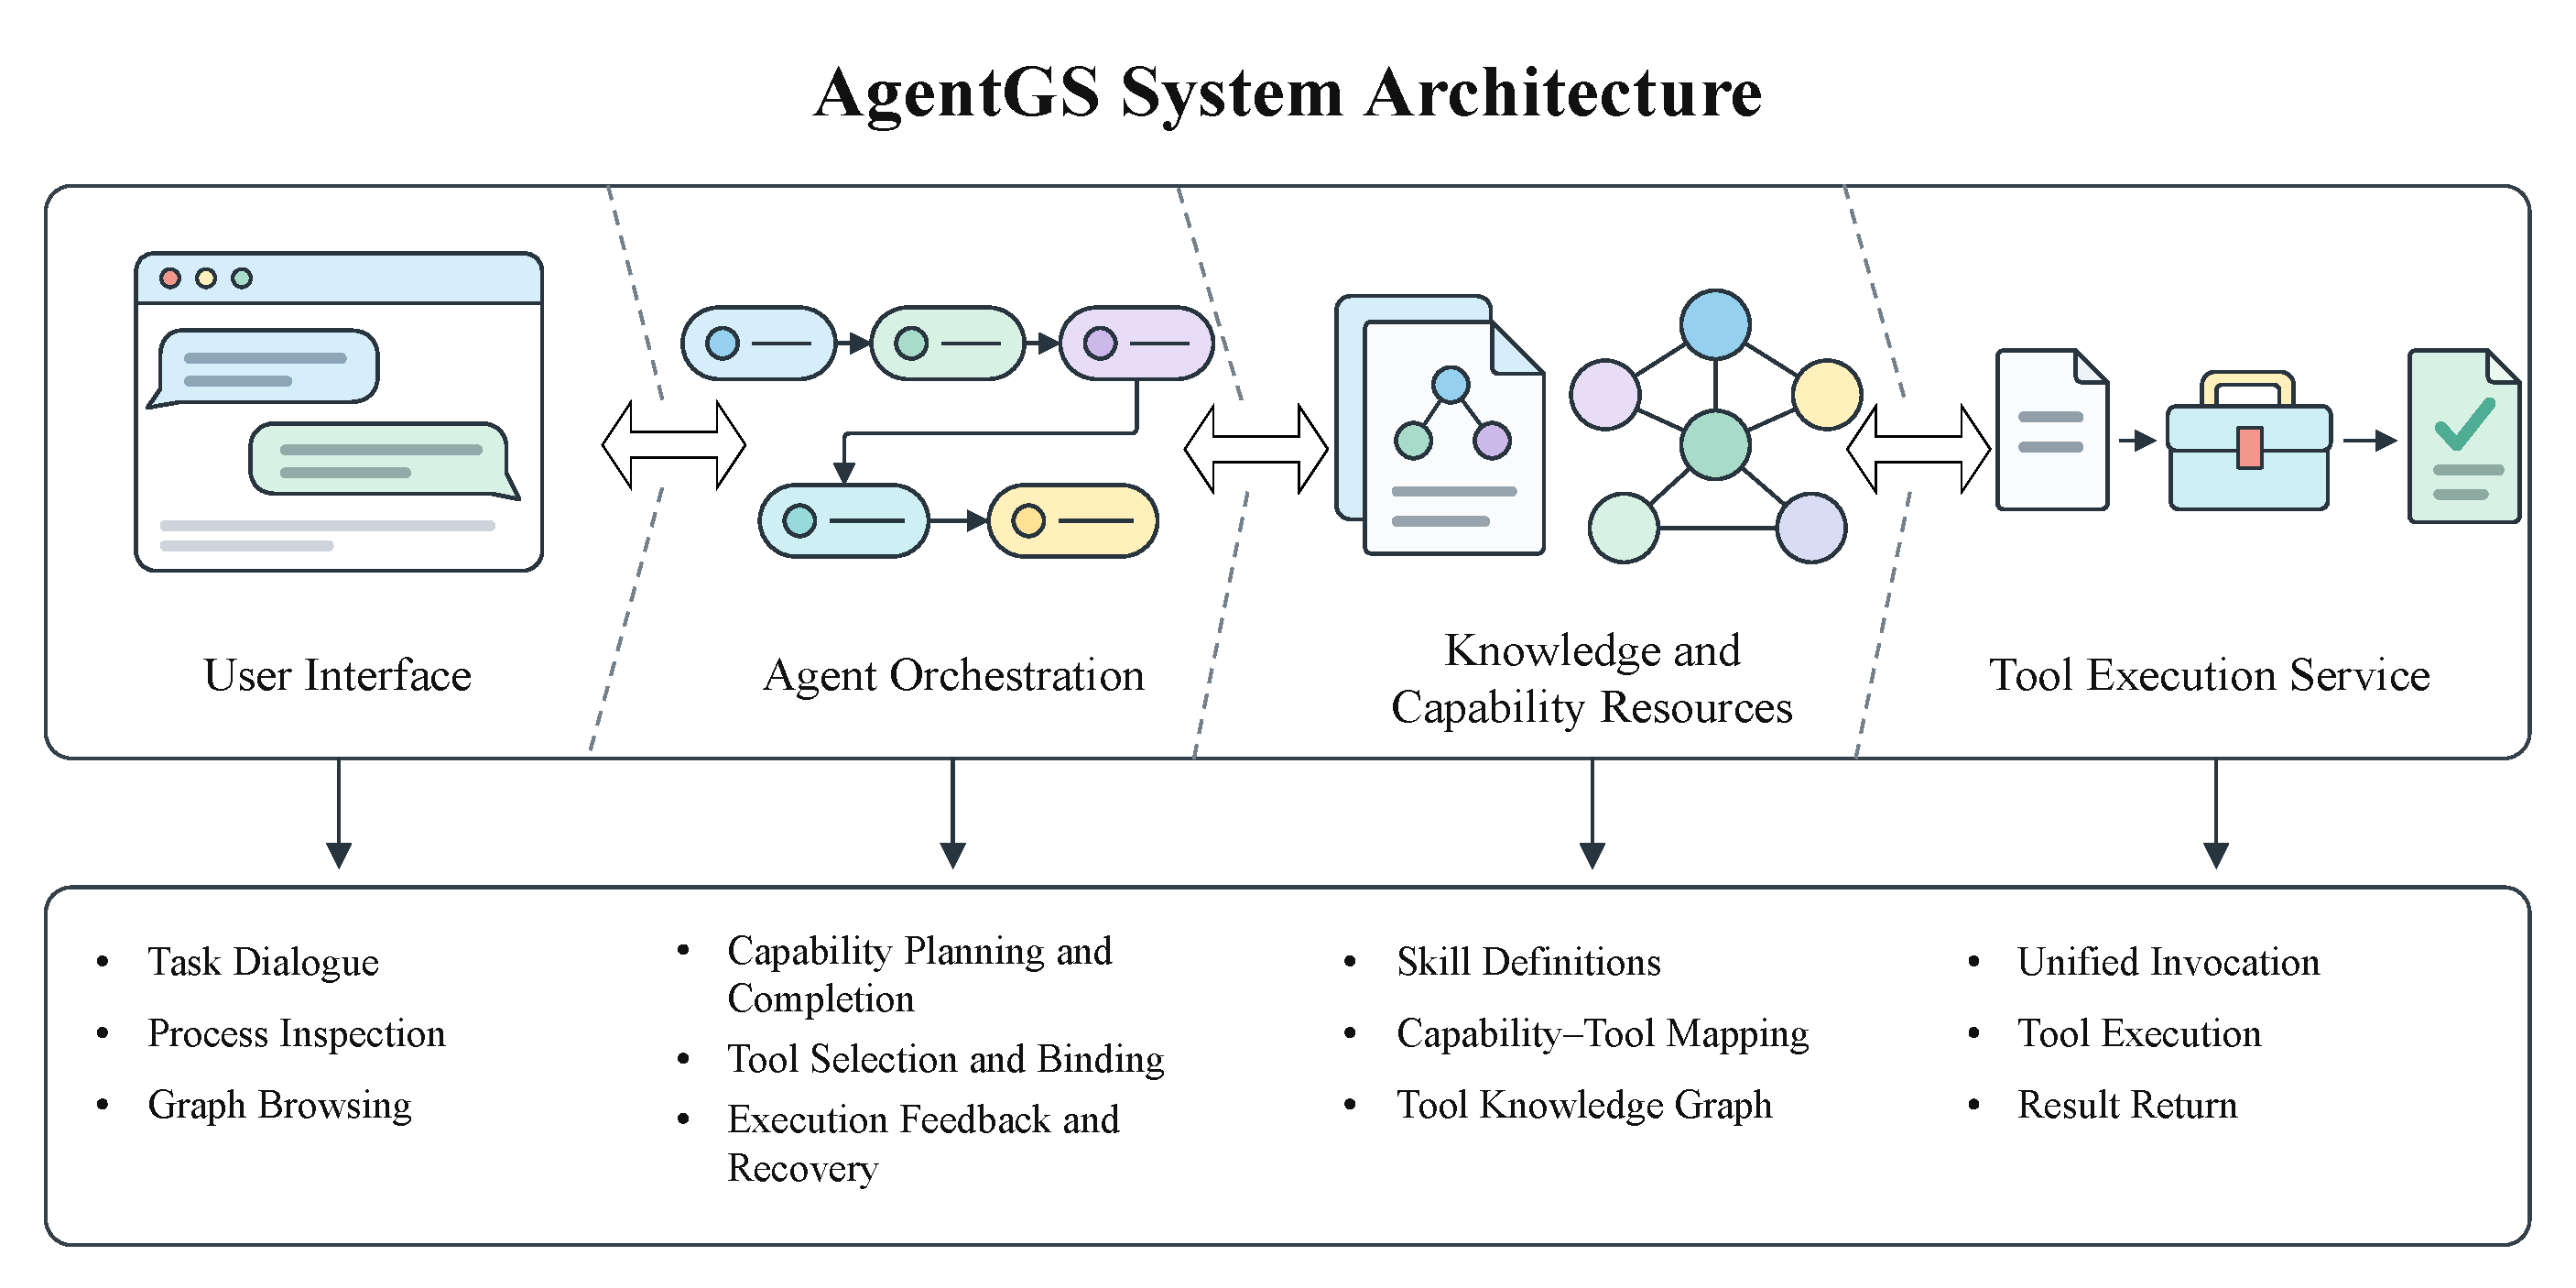
\includegraphics[width=\textwidth]{fig_architecture.pdf}
  \caption{AgentGS architecture and main functions. The system comprises an interactive frontend, an agent orchestration service, knowledge and capability resources, and a tool execution service.}
  \label{fig:architecture}
  \Description{The user interface exchanges tasks and results with orchestration. Orchestration accesses Skill definitions, capability-to-tool mappings, and tool knowledge graphs, and delegates concrete invocations to the tool execution service.}
\end{figure*}


\subsection{Separation of Planning and Execution}
The frontend accepts questions and resources and displays the returned answer and execution records. Orchestration retrieves strategies and tools, prepares capability requirements, invokes model planning, and validates the resulting instances. Knowledge resources provide Skill declarations, capability mappings, and tool descriptions. The execution service invokes a registered interface and returns its observed output or failure.

This separation allows planning to reason over declared operations while execution operates on concrete argument objects. Descriptive similarity between two tools does not by itself authorize substitution: the capability occurrence's scope and the selected interface schema still apply.

\subsection{Execution Instances and Input Bindings}
An execution step records its identity, tool, purpose, predecessor identities, literal arguments, and upstream input bindings. Optional Skill and Capability identifiers establish its declared scope. Unknown or forward dependencies and duplicate instance identities are rejected before execution.

A binding names a producing instance and a path into its observed structured output. The consumer receives the resolved value rather than an unverified description of what the producer was expected to return. Explicit references remain authoritative when arguments are repaired. This prevents a failed or inappropriate argument from being silently replaced with a convenient unrelated value.

Artifacts additionally retain provenance such as the producing step and tool. File and scalar bindings are validated according to their expected inputs. An operation on the wrong artifact may still execute successfully, which is why invocation success and reference-answer correctness are tracked separately.

\subsection{Recovery and Reuse Boundaries}
When execution recovery is enabled, the runtime can use failure feedback for argument correction and another plan attempt under configured limits. Initial model-plan repair, protocol repair, transport retries, and scientific tool retries have separate counters and scopes. Exhausting a communication budget does not establish that a scientific computation has been safely replayed.

A result can be reused across plan attempts only when the instance has unchanged semantics, fully specified inputs, and verified upstream reuse identities. The current runtime permits this for an explicit set of pure scalar computations. File-backed, implicit-input, and external-data operations are rerun rather than assumed unchanged. Matching tool names or retaining the same position in a chain is insufficient to establish reuse.

With execution recovery disabled, the first failed scientific execution ends that chain and answer generation reports incomplete work. Initial argument construction and validation remain available, so the intervention targets reaction to observed failure rather than removal of ordinary execution checks.

\subsection{Knowledge Integration and Process Inspection}
Integrating a tool registers its identifier, parameter schema, and input/output information, then associates it with relevant capabilities. A Skill supplies the strategy-specific dependency and implementation constraints. Runtime selection checks those declarations together with tool availability and the task's concrete inputs.

The interface exposes plans, invocation inputs and outputs, execution states, and failure feedback. Tool-graph browsing presents registered tools and associations as retrieval and inspection aids. These associations do not supersede capability dependencies or establish valid argument flow. Retained histories make it possible to inspect whether the intended file was read, whether the correct upstream value was consumed, and which attempts contributed to the final answer.

\section{GeoToolEval}
\label{sec:benchmark}
GeoToolEval is a dataset for evaluating scientific answers and the tool workflows used to obtain them. It covers ten geoscientific research themes and pairs each task with input resources, a reference answer, and a reference invocation chain. This supports separate analysis of outcome quality, tool coverage, and invocation order within the same evaluation record.

\subsection{Evaluation Objectives and Task Design}
\label{sec:benchmark-design}
Scientific tool use involves more than selecting a function with a relevant description. An agent must identify the intended data, instantiate the analysis with appropriate parameters, and propagate results to later operations. GeoToolEval includes tasks that exercise these requirements at different orchestration lengths.

Single-step tasks assess resource identification, parameter determination, and invocation under a registered interface. Multistep tasks additionally require composing operations and using intermediate results. For example, if a question requests the mean of a composite raster, independently computing means of the input rasters does not establish that the requested artifact was produced and analyzed. The answer and the tool trace expose different aspects of this distinction.

Tasks span three-dimensional Earth structure, geoscientific big-data analysis, critical minerals, climate change, energy resources, the global ocean carbon cycle, the deep-time biosphere, carbon capture and storage, remote sensing, and natural-disaster event statistics. This breadth covers different data objects and analytical operations. The themes are not equally sized: their counts reflect resource availability and screening outcomes.

\subsection{Task Sources and Construction}
\label{sec:benchmark-construction}
The construction combines two sources of tasks.

\paragraph{Adapted question-answer tasks.}
Questions selected from existing resources retain their source questions and reference answers, while the required operations are mapped to the registered tool interfaces. Geoscientific big-data analysis includes 40 selected GeoQuestions1089 tasks. Remote sensing includes 49 of Earth-Bench's 248 tasks~\cite{feng2026earthagent}, retaining questions, choices, and answers. Critical-mineral and climate-change tasks are selected from \nolinkurl{habitable_earth_dataset} by theme.

\paragraph{Tasks derived from scientific data.}
These tasks specify identifiable objects, variables, and computational relationships. Reference results are obtained through corresponding processing and calculations. Sources include Earth-structure models and earthquake catalogs, mineral and energy inventories, ocean-carbon observations, paleobiological data, synthetic carbon-storage monitoring data, and disaster-event records. Table~\ref{tab:benchmark} identifies the sources by theme; Appendix~\ref{app:dataset-details} gives further construction details.

\paragraph{Reference workflows and record format.}
Each evaluation record contains a natural-language question, resource locators, a reference answer, an answer type, and reference calls. A call identifies the registered tool, its parameters, and relevant input/output information. The reference chain expresses one implementation of the requested analysis under the exposed interfaces. Existing tasks retain source identifiers or locators, and data-derived tasks retain derivation records and computational scripts.

Interface adaptation determines the reference-chain length. A tool wrapper can encapsulate several processing operations in one invocation; therefore, source-dataset labels such as single-tool or multitool cannot be transferred without examining the registered interfaces.

\paragraph{Quality control.}
Construction checks source traceability, required fields, tool-name and parameter consistency, and sample execution. For data-derived tasks, retained calculations support recalculation of reference quantities. For adapted tasks, source answers provide an independent record of the target output. These checks have different scopes: a parseable invocation is not proof of scientific correctness, and successful sample execution does not certify all records. Construction validation is kept separate from the complete benchmark evaluation.

\subsection{Dataset Composition}
\label{sec:benchmark-composition}
GeoToolEval contains 603 evaluation records: 424 have one reference invocation, 119 have two or three, and 60 have at least four. Its 179 multistep records constitute 29.68\% of the dataset.
% DOCX paragraphs 119--119, table 1. All counts are copied from the source.
\begin{table*}[t]
  \caption{GeoToolEval task sources and reference tool-invocation chain lengths. Counts refer to evaluation records.}
  \label{tab:benchmark}
  \centering
  \begin{tabularx}{\textwidth}{@{}p{0.25\textwidth}Xrrrr@{}}
    \toprule
    Task theme & Main data or question sources & 1 step & 2--3 & $\geq4$ & Total \\
    \midrule
    Three-dimensional Earth structure & LITHO1.0, SEMUCB-WM1, USGS earthquake catalog & 85 & 15 & 0 & 100 \\
    Geoscientific big-data analysis & Selected GeoQuestions1089 subset & 40 & 0 & 0 & 40 \\
    Critical minerals & Habitable-Earth questions; MRDS and cross-theme climate data & 44 & 14 & 0 & 58 \\
    Climate change & Habitable-Earth questions; paleoclimate, GISTEMP, SSP, and cross-theme mineral data & 31 & 16 & 1 & 48 \\
    Energy resources & MRDS, GEM, OPSD, World Bank, and population data & 100 & 0 & 0 & 100 \\
    Global ocean carbon cycle & SOCAT, GLODAP, SNAPO-CO$_2$ & 100 & 0 & 0 & 100 \\
    Deep-time biosphere & BioDeepTime & 12 & 7 & 5 & 24 \\
    Carbon capture and storage & Synthetic SCCS-OFPOSDU CCS--MRV data & 12 & 5 & 7 & 24 \\
    Remote sensing & Selected Earth-Bench subset & 0 & 7 & 42 & 49 \\
    Natural-disaster event statistics & EM-DAT International Disaster Database & 0 & 55 & 5 & 60 \\
    \midrule
    \textbf{Total} & & \textbf{424} & \textbf{119} & \textbf{60} & \textbf{603} \\
    \bottomrule
  \end{tabularx}
\end{table*}


The critical-mineral and climate-change themes share nine cross-theme questions included in both themes. Thus, 603 denotes evaluation records rather than 603 distinct question texts. The main score weights records equally, so these repeated questions contribute through both theme assignments.

A step denotes a reference tool invocation, not an elementary scientific operation or a direct measure of scientific difficulty. Energy-resource and ocean-carbon tools, for example, can perform multiple internal operations within one call. Chain-length strata characterize orchestration demands under the current interfaces. They should be interpreted jointly with domain and wrapper design.

Long chains are unevenly distributed across themes. Remote sensing accounts for 42 of the 60 records with at least four reference calls. Consequently, changes across chain-length groups can also reflect domain-specific inputs and tools. We preserve both domain and chain-length views rather than treating either as a controlled difficulty scale.

\subsection{Evaluation Metrics}
\label{sec:metrics}
We score each record separately and average over the declared evaluation population, retaining failures. The three metrics below distinguish final-answer agreement, successful-tool coverage, and relative invocation order.

\paragraph{Final Answer Score (FAS).}
FAS lies in $[0,1]$ and preserves partial credit. Scoring depends on answer type: choice normalization for multiple-choice answers, matching rules for dates and identifiers, numerical tolerances for scalar quantities, item matching for multiple values or text items, and field-level comparison for structured answers. Empty answers receive zero. For $N$ records,
\begin{equation}
\overline{FAS}=\frac{1}{N}\sum_{i=1}^{N}FAS_i.
\label{eq:fas}
\end{equation}
The main experiment uses $N=603$. Domain and chain-length groups average their own records. This record-weighted mean is distinct from a domain-balanced macro-average or the rate of fully correct answers.

\paragraph{Tool Selection F1 (TSF1).}
Let $G_i$ be the reference sequence and $A_i$ the actual successful-call sequence for record $i$. Calls are matched one to one by tool name, treating the two sequences as multisets and retaining multiplicity. If $m_i$ calls match,
\begin{equation}
\mathrm{TSF1}_i=\frac{2m_i}{|G_i|+|A_i|}.
\label{eq:tsf1}
\end{equation}
This is the harmonic mean of successful-call precision and reference-call recall. Missing tools, irrelevant successful calls, and repeated successful invocations affect the score. Two required calls to the same tool remain two occurrences.

\paragraph{Tool Order Score (TOS).}
The longest common subsequence measures preservation of relative order:
\begin{equation}
\mathrm{TOS}_i=\frac{\mathrm{LCS}(G_i,A_i)}{|G_i|}.
\label{eq:tos}
\end{equation}
For reference order read--filter--count and actual order read--count--filter, TSF1 is 1 while TOS is $2/3$. Extra calls do not necessarily lower TOS, which is why it is reported with TSF1.

Both process metrics are zero when no invocation succeeds. Failed invocations do not enter the successful-call sequence, but failed tasks remain in the average. All three metrics are reported separately; we do not combine them into a single measure of scientific correctness.

\subsection{Interpreting Answer and Process Scores}
A reference chain records one solution under the available interfaces. An alternative valid implementation may have lower name-based process scores, while a chain with the expected names and order can still consume the wrong artifacts or use incorrect parameters. TSF1 and TOS therefore measure agreement with reference workflows rather than semantic equivalence of arbitrary analyses.

The metrics support complementary questions. FAS measures whether the returned answer matches the reference. TSF1 identifies omissions and excess successful calls relative to the reference chain. TOS measures whether matched tools occur in a compatible relative order. Explaining why an answer is wrong, or whether a different workflow is valid, requires inputs, outputs, and dependency traces in addition to these aggregates.

% DOCX paragraph 130.
\section{Experiments}
\label{sec:experiments}

% DOCX paragraph 131.
We evaluate AgentGS's overall performance and the contribution of its components through baseline comparisons and ablations. The experimental analysis also considers generalization to new combinations of existing capabilities and substitution of tools implementing the same capability, together with runtime costs. Finally, execution cases are used to examine performance differences and causes of failure. \drafttodo{generalization and runtime-cost results mentioned in the initial draft are to be supplied}.

% DOCX paragraph 132.
\subsection{Tasks and Experimental Setup}
\label{sec:experimental-setup}

% DOCX paragraph 133.
\paragraph{Data and evaluation scope.}
The main experiment uses all 603 GeoToolEval records. Ablations use a fixed subset of 57 records. All GeoToolEval experiments evaluate final answers with the FAS defined in Section~\ref{sec:metrics}, averaged over their respective evaluation sets with failures retained. To analyze workflow complexity, the main experiment additionally groups results by reference-chain length. The ablation subset is described in Section~\ref{sec:ablations}.

% DOCX paragraph 134. Model labels are retained as reported in the source.
\paragraph{Run configuration.}
We use GPT-5.6 Terra as the backbone and compute results from the raw records of AgentGS's first complete run over all 603 records, retaining both partial-credit and failed cases.

% DOCX paragraph 135.
\paragraph{Baselines.}
We compare scientific agents and language models. Agent baselines include GeoAgent~\cite{chen2024geoagent} and Earth-Agent~\cite{feng2026earthagent}. Both use GPT-5.6 Terra, as does AgentGS, to compare different agent systems with the same backbone. Language-model baselines include DeepSeek V4 Pro, GPT-5.6 Terra, GPT-5.4, Qwen-Plus, and GeoGPT. These compare direct language-model answers with answers obtained by agents using tools.

% DOCX paragraph 136.
\subsection{Main Results and Baseline Comparison}
\label{sec:main-results}

% DOCX paragraphs 137--139 and table 2.
Table~\ref{tab:main-results} reports mean FAS for AgentGS and the baselines. AgentGS achieves 0.8731, exceeding GeoAgent's 0.7804. It also outperforms the same GPT-5.6 Terra backbone answering directly, which scores 0.3137, and the other language-model baselines. We next analyze task strata and ablations to examine performance across tasks and the contributions of capability composition, hypergraph completion, and execution mechanisms.

\begin{table}[t]
\caption{GeoToolEval baseline comparison. AgentGS process metrics are per-record averages from the present 603-record end-to-end experiment; FAS values are retained from the source manuscript. Direct-answer language models have no tool traces; their process metrics are not applicable (---).}
\label{tab:main-results}
\centering
\begin{tabularx}{\columnwidth}{@{}Xrrr@{}}
\toprule
Method & FAS & TSF1 & TOS \\
\midrule
AgentGS (GPT-5.6 Terra) & \textbf{0.8731} & 0.9170 & 0.9166 \\
GeoAgent (GPT-5.6 Terra) & 0.7804 & 0.8663 & 0.7911 \\
EarthAgent (GPT-5.6 Terra) & 0.0862 & 0.1182 & 0.1390 \\
DeepSeek V4 Pro & 0.5162 & --- & --- \\
GPT-5.6 Terra & 0.3137 & --- & --- \\
GPT-5.4 & 0.3069 & --- & --- \\
Qwen-Plus & 0.2918 & --- & --- \\
GeoGPT & 0.2500 & --- & --- \\
\bottomrule
\end{tabularx}
\end{table}


% DOCX paragraph 140.
\paragraph{Task complexity and domain differences.}
Grouped by reference-chain length, AgentGS achieves mean FAS values of 0.9425 for single-step tasks, 0.7557 for two- to three-step tasks, and 0.6167 for tasks with at least four steps. Figure~\ref{fig:performance} reports results by domain. Longer chains are concentrated in remote sensing, creating overlap between chain-length and domain factors. Performance differences should therefore be interpreted using both groupings.

% DOCX paragraph 141 and embedded image 4.
\begin{figure*}[t]
  \centering
  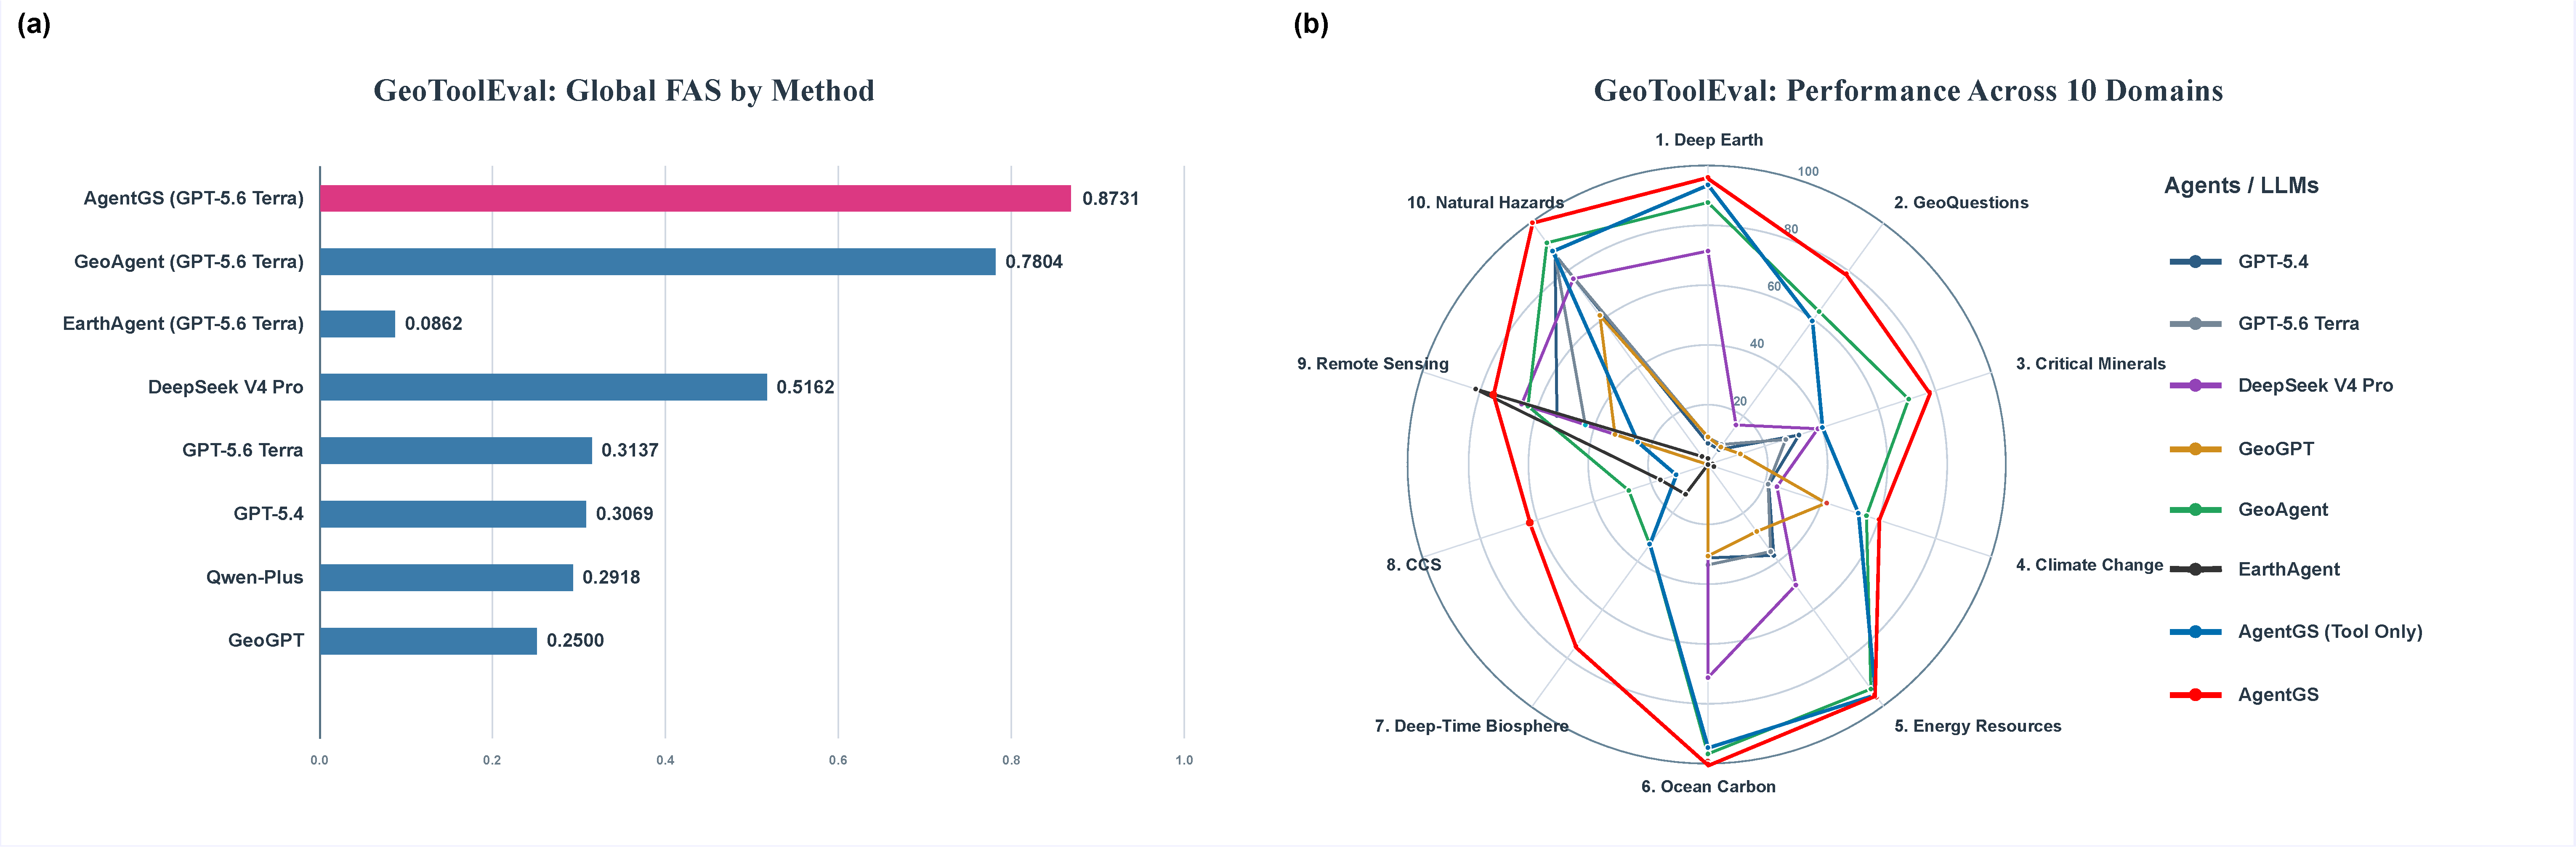
\includegraphics[width=\textwidth]{performance.pdf}
  \caption{Overall and domain-specific performance of AgentGS and baselines on GeoToolEval: (a) mean FAS across all evaluation records; (b) mean FAS across the ten geoscientific domains.}
  \label{fig:performance}
  \Description{A horizontal bar chart compares mean FAS for AgentGS, two agent baselines, and five language models. A radar chart presents performance across ten geoscientific domains.}
\end{figure*}


% DOCX paragraph 143.
\subsection{External Evaluation on GeoBenchX}
\label{sec:external-evaluation}

% DOCX paragraph 144.
To assess applicability in a different tool environment, we conduct an external evaluation on GeoBenchX~\cite{krechetova2025geobenchx}. We integrate its official tool set and separately construct corresponding Skills and Capabilities. Capabilities are defined from tool functions and input/output requirements, strategy dependencies are organized, and tool mappings are established. AgentGS then performs task planning and tool orchestration.

% DOCX paragraph 145. All experimental fields below were placeholders in the source.
The experiment uses \drafttodo{number of tasks} tasks and compares against \drafttodo{baseline method}. AgentGS and the baseline use \drafttodo{AgentGS backbone and version} and \drafttodo{baseline backbone and version}, respectively, under \drafttodo{experimental conditions actually held constant}. Evaluation is performed by \drafttodo{judge model and score aggregation} using GeoBenchX's reference-solution matching criterion: scores of 0, 1, and 2 indicate a mismatch, a partial match, and a match, respectively. We report mean score and full-match rate. These metrics are computed separately from GeoToolEval FAS.

% DOCX paragraph 146.
As shown in Table~\ref{tab:external-results}, AgentGS's mean score is \drafttodo{value}, versus \drafttodo{value} for the baseline, a difference of \drafttodo{difference} points. Their full-match rates are \drafttodo{percentage} and \drafttodo{percentage}, a difference of \drafttodo{difference} percentage points. \drafttodo{principal comparative conclusion supported by the actual results}. These results provide evidence of AgentGS's performance in an external benchmark after integrating its official tools and constructing dedicated Skills and Capabilities.

% DOCX paragraphs 147--147 and table 3.
\begin{table}[t]
\caption{Evaluation results on GeoBenchX. Both methods use GPT-5.6 Terra.}
\label{tab:external-results}
\centering
\begin{tabularx}{\columnwidth}{@{}Xrr@{}}
\toprule
Method & Mean score & Full-match \\
 & $(0$--$2)\uparrow$ & rate $(\%)\uparrow$ \\
\midrule
ReAct & 1.1980 & 53.47 \\
AgentGS & \textbf{1.3762} & \textbf{62.87} \\
\bottomrule
\end{tabularx}
\end{table}


% DOCX paragraph 148.
\subsection{Ablation Experiments}
\label{sec:ablations}

% DOCX paragraph 149.
Ablations use 57 GeoToolEval records covering all ten geoscientific domains. There are 22 single-step records, 20 with two or three steps, and 15 with at least four steps; multistep records comprise 61.40\% of the subset. All configurations are evaluated on the same subset, with the full method on that subset serving as the reference. Each experiment disables or changes one mechanism. We compare mean FAS over the full subset and over its multistep records to analyze hierarchical planning, missing-capability completion, and execution mechanisms.

% DOCX paragraph 150.
\paragraph{Hierarchical planning and predecessor expansion.}
A1 retains the same strategy, dependency, and tool information but plans directly at the tool level, providing a structural control for hierarchical decision making. A2 retains initial capability selection and dependency declarations while disabling automatic expansion of mandatory predecessors. It tests the contribution of explicitly inserting prerequisite operations. Since subsequent completion may restore omitted predecessors, the analysis also records plan changes and compensatory insertions.

% DOCX paragraph 151.
\paragraph{Missing-capability completion.}
A3 retains gap diagnosis but disables automatic insertion of supporting capabilities, including directed bridging, to test the overall contribution of independent completion. A4 disables only directed bridging while retaining other completion mechanisms, testing the additional benefit of connecting branches from inactive Skills. Both ablations are analyzed alongside required-operation coverage, dependency satisfaction, and actual use of upstream artifacts.

% DOCX paragraph 152.
\paragraph{Tool selection and execution recovery.}
A5 retains capability requirements, instance-specific candidate scopes, and execution validation, but selects the first valid candidate in a predefined fixed order. This tests the contribution of selection optimization. A6 disables local recovery after execution failures while retaining planning, tool selection, and input binding before the first execution. It tests the contribution of recovery to task completion.

% DOCX paragraphs 153--154 and table 4.
\begin{table}[t]
\caption{Earlier component comparison on 57 records, including 35 multistep records. A1 is a partial control; A2 did not activate its intended intervention.}
\label{tab:ablation}
\centering
\begin{tabularx}{\columnwidth}{@{}Xrr@{}}
\toprule
Configuration & FAS & Multistep FAS \\
\midrule
Full & 0.6387 & 0.5333 \\
A1: Flat planning & 0.4748 & 0.4095 \\
A2: w/o predecessor expansion & 0.4760 & 0.4095 \\
A3: w/o automatic completion & 0.4624 & 0.3802 \\
A4: w/o directed bridging & 0.6160 & 0.4913 \\
\bottomrule
\end{tabularx}
\end{table}


% DOCX paragraph 155.
\paragraph{Ablation analysis.}
Hierarchical planning, predecessor expansion, and independent completion all have substantial effects. Relative to the full method, A1's direct tool-level planning reduces overall mean FAS by 25.82 percentage points and multistep FAS by 24.74 points. This supports first determining capabilities and their dependencies, then selecting tools. Disabling predecessor expansion (A2) and independent completion (A3) reduces overall mean FAS by 24.43 and 23.94 points, respectively, and multistep FAS by 27.43 and 26.88 points. The larger multistep declines indicate that completing mandatory prerequisites and missing capabilities is particularly important for multistep tasks.

% DOCX paragraph 156.
With the other completion mechanisms retained, disabling directed bridging alone (A4) reduces overall mean FAS by 2.27 points and multistep FAS by 4.20 points. Directed bridging therefore adds benefits beyond the existing completion mechanisms, with larger benefits on multistep tasks. Compared with disabling all independent completion, this result also indicates that bridging is an effective complement to the broader completion mechanism.

% DOCX paragraph 157.
Execution mechanisms have different effects. Disabling execution recovery (A6) reduces overall and multistep FAS by 4.15 and 7.20 points, respectively, suggesting that local recovery reduces the impact of execution failures on task completion. In contrast, disabling tool-selection optimization (A5) slightly increases overall mean FAS from 0.6387 to 0.6415, while reducing multistep FAS from 0.5333 to 0.5184. These results support its benefit on multistep tasks, but do not show a consistent improvement in overall score.

\subsection{Case Study}
\label{sec:case-study}

We use an illustrative case to show how the system combines capabilities from different Skills, fills missing steps, and forms concrete tool calls. Consider the task: given several remote-sensing rasters of the same region, create and return a pixel-wise mean composite, compute the mean of its valid pixels, state whether that mean exceeds a given reference value, and report the difference. The inputs represent the same variable, their spatial grids are aligned, and the reference value uses the same units as the raster values.

\begin{figure*}[t]
  \centering
  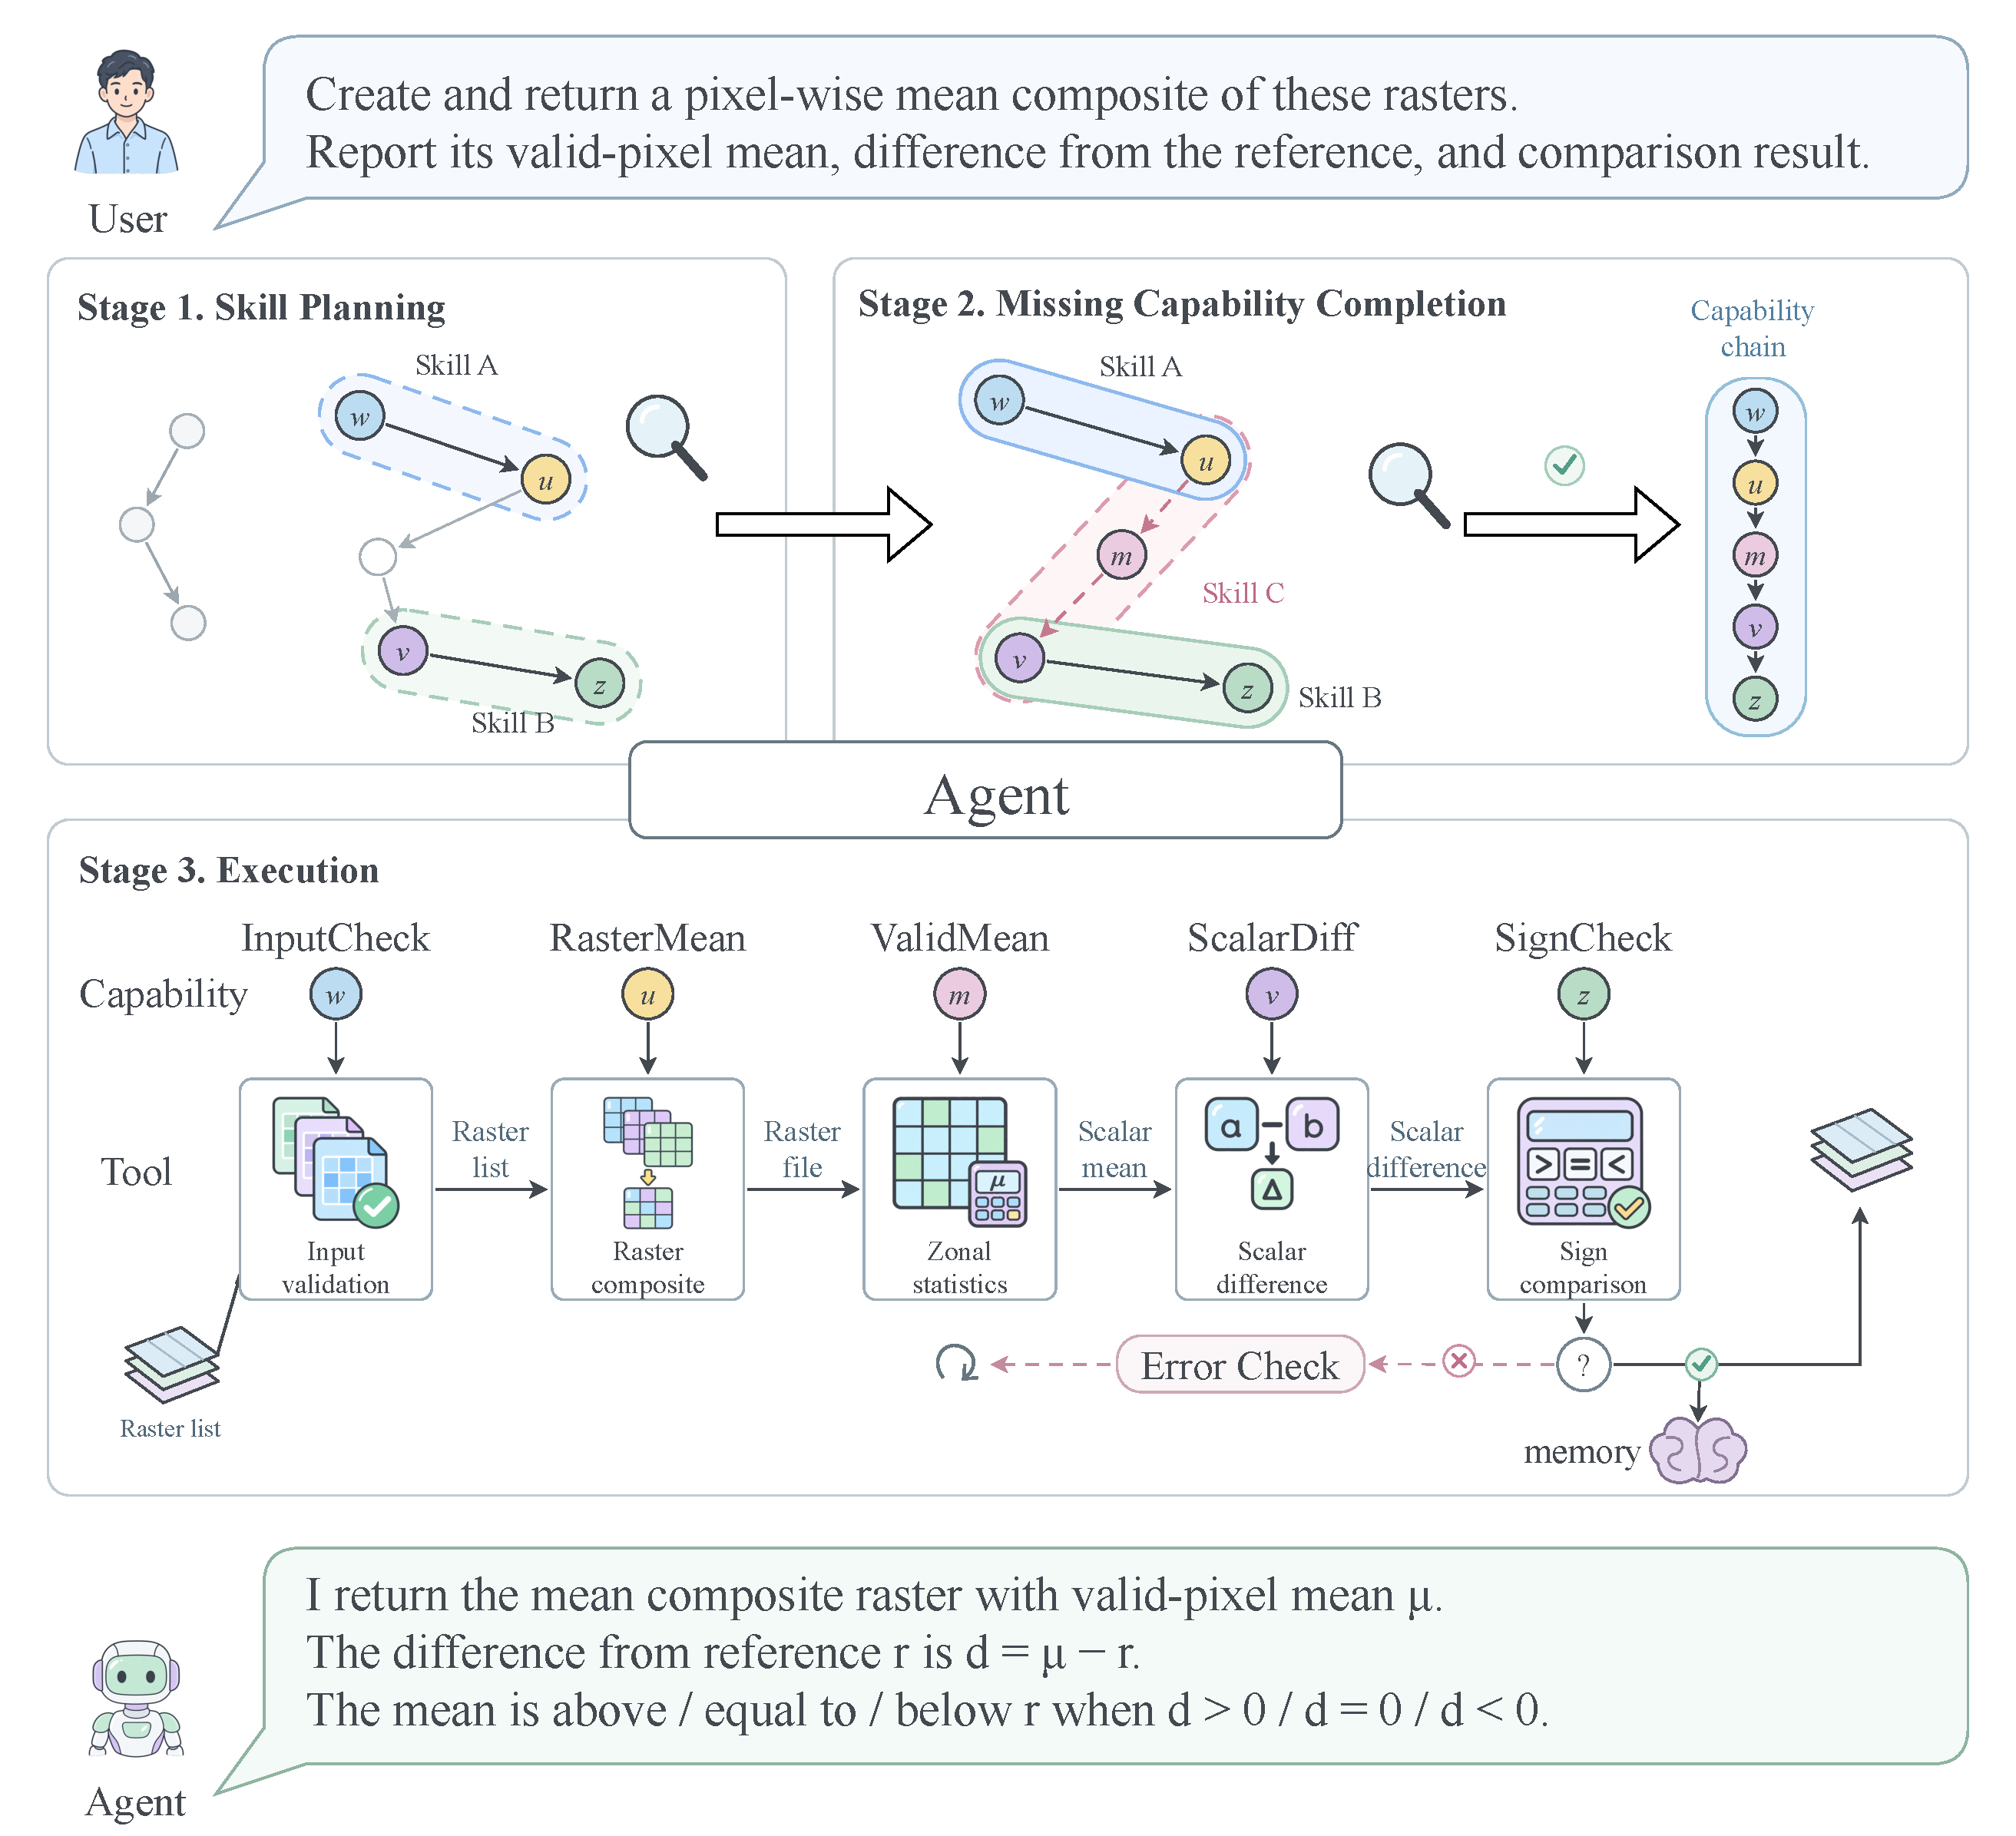
\includegraphics[width=0.83\textwidth]{fig_case_study.pdf}
  \caption{Cross-Skill capability composition and tool execution. Stage 1 selects $w\to u$ from Skill $A$ and $v\to z$ from Skill $B$. Stage 2 inserts valid-pixel mean statistics $m$ using Skill $C$'s $u\to m\to v$ branch. Stage 3 grounds the five-step workflow in tool calls, propagates intermediate artifacts, and returns the composite raster, mean, difference, and comparison relation. The workflow is a mechanism illustration.}
  \label{fig:case-study}
  \Description{The case proceeds from two selected Skill fragments to a completed five-capability chain and corresponding input-validation, raster-compositing, zonal-statistics, scalar-differencing, and sign-comparison tools.}
\end{figure*}


\emph{Skill Retrieval} returns only RasterCompose (Skill $A$) and ReferenceCompare (Skill $B$). \emph{Skill Planning} selects InputCheck ($w$) and RasterMean ($u$) from the former, and ScalarDiff ($v$) and SignCheck ($z$) from the latter. InputCheck verifies the variable and spatial-grid requirements. RasterMean produces the mean raster from the validated image list, giving $w\to u$. ScalarDiff returns the difference between the value under comparison and the reference; SignCheck uses that difference to determine whether the value is above, equal to, or below the reference, giving $v\to z$. Hypergraph Composition expands mandatory predecessors declared by the selected strategies and retains provenance and candidate-tool scopes. At this stage, the plan consists of two disconnected fragments: compositing produces a raster file, whereas differencing requires a numerical input. The operation computing the mean of the composite is still missing.

Using $u$ and $v$ as shared endpoints, Missing Capability Completion retrieves $u\to m\to v$ from inactive RasterDiff (Skill $C$), where ValidMean ($m$) extracts the mean of valid pixels from the composite. Here, RasterDiff means differencing a statistic of the composite against a reference value. The query explicitly requires the mean statistic; Skill $C$ supplies reusable dependencies and usage constraints connecting it to the preceding and following operations. Under this example's assumptions, it is the only candidate for the ordered endpoint pair satisfying prerequisite, type, tool-availability, and acyclicity requirements: $u$'s raster output is compatible with $m$'s input, and $m$'s numerical output is compatible with $v$. Insertion preserves $u$'s original constraints, adds $m$, and updates $v$'s dependencies, candidate-tool scope, and input bindings. Existing dependencies $w\to u$ and $v\to z$ remain. Recomposition and dependency verification connect the fragments into input validation, mean compositing, valid-pixel mean statistics, scalar differencing, and sign comparison: $w\to u\to m\to v\to z$.

Tool Grounding then selects validation, compositing, statistics, differencing, and sign-comparison tools within each instance's candidate scope and parameter constraints. GeoToolKG associations guide candidate retrieval, but concrete invocations still require instance and input-compatibility checks. Grounding a bridge into calls additionally requires that $u$ and $v$ each correspond to exactly one endpoint instance and that their order agrees with the bridge direction. During execution, the validated image list is passed to the compositing tool. The statistics tool receives a list containing only the composite raster's path. The returned mean and the task's reference value are bound to differencing parameters $a$ and $b$, producing $d=a-b$. Sign comparison then compares $d$ with zero. The statistical object remains the composite created for this task, the comparison baseline remains the supplied reference, and the final relation is based on the same difference calculation.

If the zonal-statistics call fails, Failure Recovery uses the failure state and recovery rules to decide whether to retry or select an alternative within the instance's permitted scope. Completed validation and compositing steps are retained, and the composite is reused. Calls with uncertain outcomes are not automatically replayed, and later execution is suspended if recovery requires adding a capability. Once all steps succeed, Final Answer summarizes the composite raster, valid-pixel mean, difference, and comparison relation, addressing each requested output. This case illustrates that cross-Skill completion must both connect capability steps and preserve dependencies while accurately binding task inputs and intermediate artifacts to subsequent calls.

After successful execution and result verification, the five-step workflow can also be organized into a candidate CompositeCompare Skill ($D$). It parameterizes the image list and reference value as rebindable task inputs, and retains artifact dependencies and capability usage constraints. This provides a strategy description for later reuse of the composition. Applicability to other inputs and tasks requires further verification; the example does not establish a reuse benefit for the new Skill.


\section{Conclusion}
\label{sec:conclusion}
We present AgentGS and GeoToolEval for tool orchestration in Earth science. AgentGS separates reusable strategies, shared operations, and concrete implementations through a Skill--Capability--Tool representation. It composes local workflow fragments while retaining their dependencies and usage constraints, then searches the skill hypergraph for admissible operations that complete missing connections. Explicit grounding and artifact bindings connect this plan to executable scientific analysis.

GeoToolEval supplies 603 evaluation records across ten research themes, with reference answers and tool workflows that support separate measures of answer agreement, tool coverage, and invocation order. AgentGS achieves reported mean FAS of 0.8731, compared with 0.7804 for the strongest reported agent baseline, and also obtains higher aggregate process scores. The configuration study exposes answer and workflow differences while identifying limits on attributing them to individual mechanisms.

The resulting framework makes composition and completion inspectable at the level of operations, dependencies, and observed artifacts. Further evaluation should examine unseen capability combinations, controlled changes in the tool environment, and the utility of verified compositions as reusable strategies. Broader scientific reliability also requires validating task semantics and resource use beyond agreement with a reference call sequence.


\FloatBarrier
\bibliographystyle{ACM-Reference-Format}
\balance
% These entries remain in the Word reference list but are not cited in its revised body.
\nocite{wang2023voyager,liu2024toolnet,liu2024controlllm,lee2025innout}
\bibliography{references}

\end{document}
